\documentclass{beamer}
\usetheme{Madrid}

\usepackage{amsmath, amssymb, amsthm}
\usepackage{graphicx}
\usepackage{listings}
\usepackage{gensymb}
\usepackage[utf8]{inputenc}
\usepackage{hyperref}
\usepackage{gvv}

\begin{document}

\title{DISCRETE ASSIGNMENT}
\author{EE23BTECH11016 - Aditi Dure$^{*}$}
\date{}
\frame{\titlepage}

\begin{frame}
\frametitle{Question}
If $a\left(\frac{1}{b} + \frac{1}{c}\right)$, $b\left(\frac{1}{c} + \frac{1}{a}\right)$, $c\left(\frac{1}{a} + \frac{1}{b}\right)$ are in arithmetic progression (AP), prove that $a$, $b$, $c$ are also in AP.
\end{frame}

\begin{frame}
\frametitle{Solution: Theory}
\frametitle{Theory}
Common difference can be written as: 
\begin{align}
b\left(\frac{1}{c} + \frac{1}{a}\right) - a\left(\frac{1}{b} + \frac{1}{c}\right) &= c\left(\frac{1}{a} + \frac{1}{b}\right) - b\left(\frac{1}{c} + \frac{1}{a}\right)  \\ \implies
(b - a)\brak{\frac{1}{a} + \frac{1}{b} + \frac{1}{c}} &= (c - b)\brak{\frac{1}{a} + \frac{1}{b} + \frac{1}{c}} \\ \implies
b - a &= c - b  
\end{align}
Hence proved that $a$, $b$, $c$ are in AP. 
\end{frame}

\begin{frame}
\frametitle{Theory}
%add table
\begin{table}[!h]
\begin{tabular}{|c|c|c|} 
      \hline
\textbf{Variable}& \textbf{Description}& \textbf{Value}\\\hline
         $x(n)$& general term of sequence&$2^{n} u(n)$\\\hline
         
    \end{tabular}

\caption{Input Parameter Table}
\label{tab:11.9.5.16.tab1}
\end{table}
\end{frame}

\begin{frame}
\frametitle{Theory}
From table \ref{tab:11.9.5.16.tab1}
\begin{align}
X(z) &= x(0)\brak{\frac{1}{1- z^{-1}}} + d\brak{\frac{z^{-1}}{(1-z^{-1})^2}} \\
&= a\left(\frac{1}{b} + \frac{1}{c}\right)\brak{\frac{1}{1- z^{-1}}} + (b - a)\brak{\frac{1}{a}  + \frac{1}{b} + \frac{1}{c}}\brak{\frac{z^{-1}}{(1-z^{-1})^2}} 
\end{align}
where $\abs{z} >1$
\end{frame}

\begin{frame}
\frametitle{Theory}
\begin{figure}[h]
    \centering
    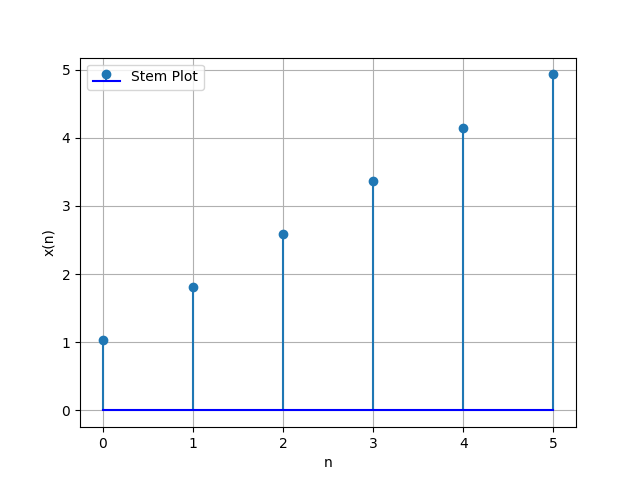
\includegraphics[width=\columnwidth]{./figs/fig1.png}
    \caption{Graph with values of $a = 3, b = 5, c = 7$ }
\end{figure}
\end{frame}

\begin{frame}[fragile]
\frametitle{C Code}
\begin{lstlisting}[language=C]
#include <stdio.h>
#include <math.h>

void linespace(int start, int stop, int step, int* n_values, double* x_values, int num_values) {
    for (int i = 0; i < num_values; ++i) {
        n_values[i] = start + i * step;
        //corresponding values of x(0) = 36.0/35 and d_x = 82.0/105
        x_values[i] = 36.0/35 + n_values[i]*82.0/105;
    }
}
int main() {
    // Define the range and step size
    int start = 0;
    int stop = 5;
    int step = 1;
\end{lstlisting}
\end{frame}

\begin{frame}[fragile]
\frametitle{C Code}
\begin{lstlisting}[language=C]


    // Calculate the number of values in the range
    int num_values = (stop - start) / step + 1;

    // Allocate arrays to store the generated values
    int n_values[num_values];
    double x_values[num_values];

    // Call the linespace function
    linespace(start, stop, step, n_values, x_values, num_values);

    // Save data to a file
    FILE* file = fopen("output.dat", "w");
\end{lstlisting}
\end{frame}

\begin{frame}[fragile]
\frametitle{C Code}
\begin{lstlisting}[language=C]
    if (file != NULL) {
        for (int i = 0; i < num_values; ++i) {
            fprintf(file, "%d %.2lf\n", n_values[i], x_values[i]);
        }

        fclose(file);
        printf("Data saved to 'output.dat'.\n");
    } else {
        printf("Error opening file for writing.\n");
    }

    return 0;
}
\end{lstlisting}
\end{frame}

\begin{frame}[fragile]
\frametitle{Python Code}
\begin{lstlisting}[language=Python]
import matplotlib.pyplot as plt
import numpy as np

# Load data from the "output.dat" file using numpy's loadtxt
data = np.loadtxt("output.dat")
# Extract n_values and y_values from the data
n_values = data[:, 0].astype(int)
x_values = data[:, 1]

# Create a stem plot
plt.stem(n_values, x_values, linefmt='|', markerfmt='o', basefmt='b', label='Stem Plot')
\end{lstlisting}
\end{frame}


\begin{frame}[fragile]
\frametitle{Python Code}
\begin{lstlisting}[language=Python]
plt.xlabel('n')
plt.ylabel('x(n)')
plt.grid(True)
plt.legend()
plt.savefig('../figs/fig1.png')
plt.show()
\end{lstlisting}
\end{frame}

\end{document}

